% 1977 年四川卷第六题(3)：(x+2)^2-(y-1)^2=0 的图象——直线 x-y+3=0 与 x+y+1=0（按源卷第 5 页图三布局）
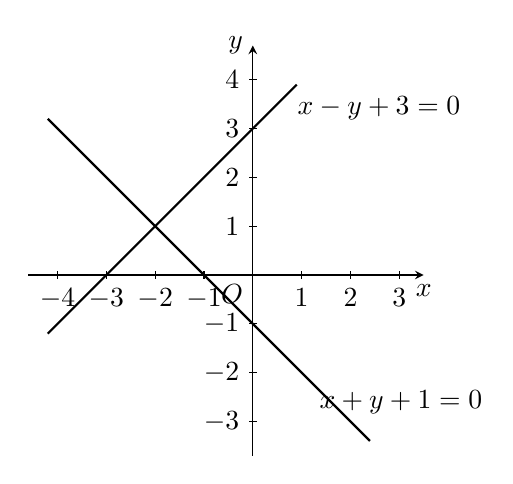
\begin{tikzpicture}[scale=0.62,>=stealth]
  \draw[->] (-4.6,0)--(3.5,0) node[below] {$x$};
  \draw[->] (0,-3.7)--(0,4.7) node[left] {$y$};
  \node[below left] at (0,0) {$O$};
  \foreach \x in {-4,-3,-2,-1,1,2,3}{
    \draw[thin] (\x,0.08)--(\x,-0.08) node[below] {$\x$};
  }
  \foreach \y in {-3,-2,-1,1,2,3,4}{
    \draw[thin] (0.08,\y)--(-0.08,\y) node[left] {$\y$};
  }
  \draw[thick] (-4.2,-1.2)--(0.9,3.9);
  \draw[thick] (-4.2,3.2)--(2.4,-3.4);
  \node[right] at (0.72,3.42) {$x-y+3=0$};
  \node[below right,inner sep=1pt] at (1.30,-2.30) {$x+y+1=0$};
\end{tikzpicture}
